\documentclass{article}
\usepackage{graphicx}
\usepackage[utf8]{inputenc}

\title{7g rapport}
\author{Henrik Flindt\\Nicolas Dyhrman\\Adrian Joensen}
\date{\today}

\begin{document}
    \maketitle
    \section{Our Plan}
        To start the game the players enter fsharpc awariLibIncomplete.fs playAwari.fsx and mono playAwari.exe.
        \\
        Visually, we decided the playerscreen should be simple and easy. Instead of pixels of beans and pits we chose to use numbers and even spaces to illustrate the board.
        \\
        When it came to the programming, we decided a list is going to represent the board.
        \\
        Since we are trying to do functional programming we thought "Okay, if we can't figure out how to use Martin's template we will just make a bunch of functions that do what needs to be done and make a main function that uses all the functions in order to run the game."
        \\
        To choose a pit the player would enter an integer between 1 to 6.
        \\
        To exit the game the players have to press ctrl c then y.
    \section{Here's What We Did}
        Below we have some of Martin's template and some of the functions that do what needs to be done.
        \\
        \textbf{clearPit:} Clears the element that corresponds to the chosen pit in the list.
        \\
        \textbf{matchOppositePit:}
        This function will give you the opposite index value on the board. So 1 and 13 is opposite of each other. This will return -1 if you give it a home value (So 0 or 7) or if a value higher than 13 or if lower than 0.
        \\
        \textbf{emptyPit:}
        This function will return a new board if one of the players has hit an empty pit. This new board is where the pit you hit and the opposite pit is both emptying out and putting it into your own home. It will return a new board and the last pit used afterwards.
        \\
        \textbf{distribute:} adds by 1 to the elements after the corresponding element.
        \\
        \textbf{printBoard:} Prints the board. We added "$|$" for clarity and "Awari" for style.
        \\
        \textbf{findWinner:} Takes the elements that correspond to the players' homes and checks who won.
        \\
        \textbf{isGameOver:} Returns true if either side is empty.
        \\
        \textbf{isHome:} Checks if the player is on his home pit.
        \\
        \textbf{getOppositePit:} Takes the opponent's beans and returns it.
        \\
        \textbf{CreateNewBoardFromHitEmptyPit:} Updates the list when a player lands on the opponent's empty pit.
        \\
        \textbf{HitEmptyPit:} Detects if the player landed on the opponent's empty pit.
        \\
        \textbf{pitEmpty:} Returns if the pit is empty.
        \\
        \textbf{reverseNumbers:} Reverses the players possible input. For example if player 1 chooses 1 it will turn to last possible input 6 because the indexes and the pit numbers don't match.
        \\
        \textbf{getMove:} Receives the players' input and check if it's a legit move.
        \\
        \textbf{turn:} Checks who's turn it is according to the rules.
        \\
        \textbf{play:} Main function that runs the whole thing.
        \\
    \section{White Box Testing}
        Here, we check if clearPit empties the element of the list if we enter index 1, 3, 7 or 13.\\
        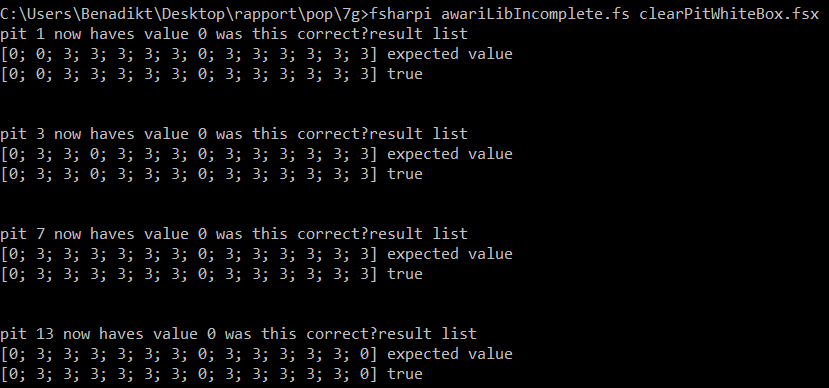
\includegraphics[scale=0.6]{clearPitWhieBox.png}
        \\
        For distribute, we check if the function does have the correct remaining beans (bolds left) from the right place(pit)
        \\
        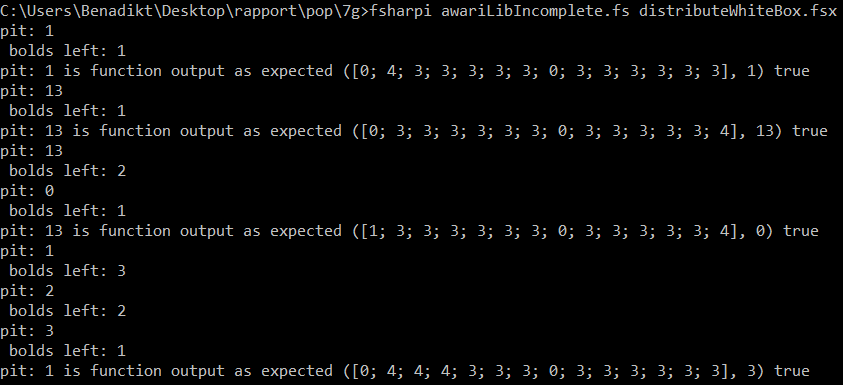
\includegraphics[scale=0.6]{distributeWhiteBox.png}
        \\
        Here, we made sure that if either player's score is higher it returns the right boolean.
        \\
        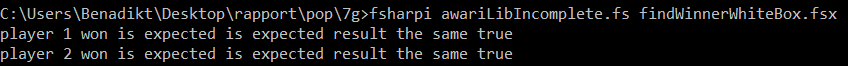
\includegraphics[scale=0.6]{findWinnerWhiteBox.png}
        \\
        Here, we check it returns correctly depending on how the list is.
        \\
        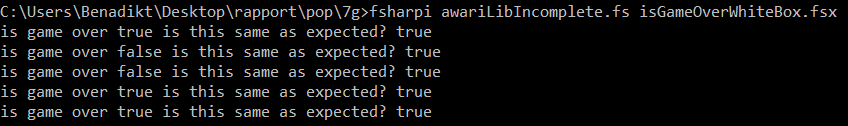
\includegraphics[scale=0.6]{isGameOverWhiteBox.png}
        \\
        This insures what happens when the players land on the home pit.
        \\
        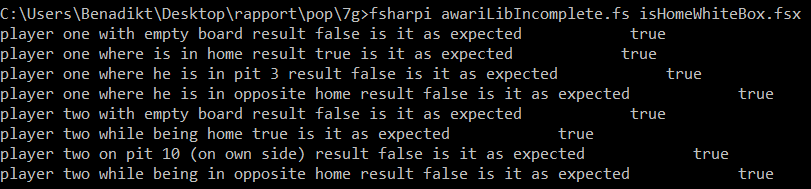
\includegraphics[scale=0.6]{isHomeWhiteBox.png}
        \\
        Here we see what getMove returns depending on the input.
        \\
        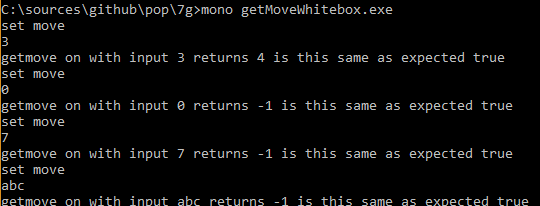
\includegraphics[scale=0.5]{getMoveWhiteBox.png}
        \\
        Checks what happens if the players land on an empty pit.
        \\
        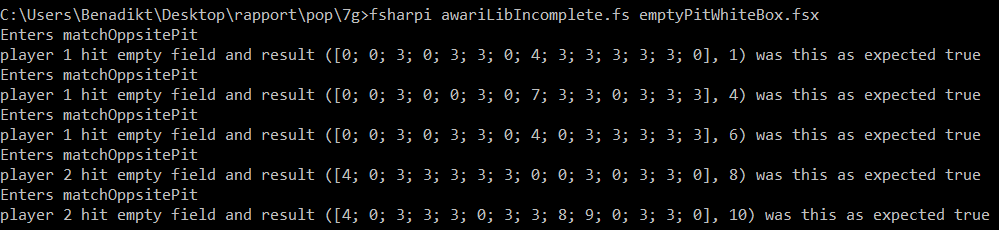
\includegraphics[scale=0.6]{emptyPitWhiteBox.png}
        \\
        This checks when player input is 1, 3, 6 and 7 returns correctly.
        \\
        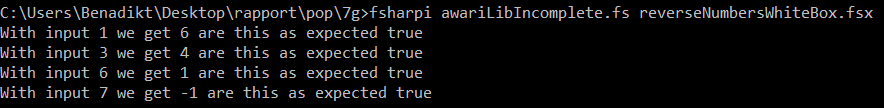
\includegraphics[scale=0.6]{reverseNumbersWhiteBox.png}
        \\
        Here, we check what happens if the pit is empty or not.
        \\
        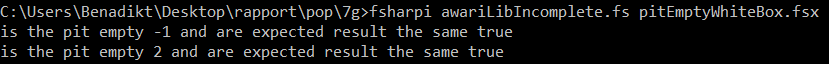
\includegraphics[scale=0.6]{pitEmptyWhiteBox.png}
        \\
    \section{Source Code}
    \begin{verbatim}
module Awari
type pit = int
type board = int list
type player = Player1 | Player2


let clearPit (l: int list) p =
    let a = l.[0..p-1]
    let b = [0]
    let c = l.[p+1..13]
    a @ b @ c

let matchOppsitePit (p: pit): pit =
  printfn "Enters matchOppsitePit"
  match p with
  | 1 -> 13
  | 2 -> 12
  | 3 -> 11
  | 4 -> 10
  | 5 -> 9
  | 6 -> 8
  | 8 -> 6
  | 9 -> 5
  | 10 -> 4
  | 11 -> 3
  | 12 -> 2
  | 13 -> 1
  | _ -> -1

let emptyPit (b: board) (p: pit): board * pit =
  printfn "Enters emptyPit"
  if p < 7 then
    let op = matchOppsitePit p
    printfn "Exit matchOppesitePit"
    let a = b.[..p-1]
    let c = [0]
    let d = b.[p+1..6]
    let home = [b.[7]+b.[p]+b.[op]+1]
    let f = b.[8..op-1]
    let g = [0]
    let h = b.[op+1..13]
    let uL = a @ c @ d @ home @ f @ g @ h
    (uL, p)
  else
    let op = matchOppsitePit p
    printfn "Exit matchOppesitePit"
    let home = [b.[0]+b.[p]+b.[op]+1]
    let a = b.[0..op-1]
    let c = [0]
    let d = b.[op+1..6]
    let e = [8..p-1]
    let f = [0]
    let g = b.[p+1..13]
    let uL = home @ a @ c @ d @ e @ f @ g
    (uL, p)

let rec distribute (l: board) (p : pit) (b : int) : board * pit =
  let a = l.[..p-1]
  let d = [l.[p]+1]
  let c = l.[p+1..] //if p = 0 && b = 1 => playerhome + zero pit + obs pit.
  if ((l.[p]=0) && (b = 1) && (not (p = 0)) && (not (p = 7))) then
    printfn "pit: %i\n bolds left: %i" p b
    emptyPit l p
  else
    let uL = a @ d @ c

    printfn "pit: %i\n bolds left: %i" p b

    if p >= 13 then
      if (b <> 1) then
        distribute uL 0 (b-1)
      else
        (uL, p)
    elif b <= 1 then
        (uL, p)
    else
        distribute uL (p+1) (b-1)

  //printfn "pit: %i\n bolds left: %i" p b



let printBoard(b: board): unit = //For printing the board a variation of the Maurits-printing-metoed seen in previus assigment.
  printfn "\n    1   2   3   4   5   6\n           <--         \n    %i | %i | %i | %i | %i | %i\n %i          Awari          %i\n    %i | %i | %i | %i | %i | %i\n" (b.Item(6)) (b.Item(5)) (b.Item(4)) (b.Item(3)) (b.Item(2)) (b.Item(1)) (b.Item(7)) (b.Item(0)) (b.Item(8)) (b.Item(9)) (b.Item(10)) (b.Item(11)) (b.Item(12)) (b.Item(13))
  //Spacial locality? What is that...

let findWinner (b : board) : string =
  let player1Pit = b.[7]
  let player2Pit = b.[0]

  if(player1Pit > player2Pit) then
    sprintf "Player 1 won with %i points, while Player 2 had %i" player1Pit player2Pit
  elif(player1Pit < player2Pit) then
    sprintf "Player 2 won with %i points, while Player 1 had %i" player2Pit player1Pit
  else sprintf "Both players are drawn with a score of %i:%i!"player1Pit player2Pit



let isGameOver (b : board) : bool =
  if b.IsEmpty then
    true
  else
    // checker om player1's side består af 0 pinde
    let player2gameover = List.forall (fun elem -> elem = 0) b.[1..6]
    // checker om player2's side består af 0 pinde
    let player1gameover = List.forall (fun elem -> elem = 0) b.[8..13]

    // Returner resultater fra udregninger ovenfor
    if player1gameover then
      player1gameover
    elif player2gameover then
      player2gameover
    else
      false

let isHome (b : board) (p : player) (i : pit) : bool =

  // Hvis listen er tom er der ingen hjem derfor return false
  if b.IsEmpty then
    false
  else
    // Finder ud af hvor stort halvdelen af boardet er
    let halfBoardLen = b.Length / 2

    // Plyayer 1's hjem er det første elem (kan også udregnes som 0) men det samme som halvdelen af boardets længde minus halvdelen af boardets længde
    let player1Home = halfBoardLen - halfBoardLen

    // Player 2's hjem kan udregnes ved at halvere boardets længde (kan også bare laves som halfBoardLen)
    let player2Home = b.Length - halfBoardLen

    // Checker hvilken spiller der skal tjekkes om er hjemme
    match p with
    | Player1 ->
      if i = 7 then
        true
      else
        false

    | Player2 ->
      if i = 0 then
        true
      else
        false

let getOppositePit (bLen : int) (i : pit) (p : player) : pit =
  match p with
  | Player1     -> (bLen / 2) - abs i
  | Player2     -> (bLen / 2) + abs i


// pit 1 = player 1's pit
// pit 2 = player 2's pit
let CreateNewBoardFromHitEmptyPit (board : board) (pit1 : pit) (pit2 : pit) (p : player) : board =
  printfn "Player 1"

  match p with
  | Player1 ->
    let newHomeValue = board.[7] + board.[pit2] + 1
    let a = board.[0 .. (pit1-1)]
    let b = [0]
    let c = board.[(pit1+1) .. 6]
    let d = [newHomeValue]
    let e = board.[8 .. (pit2-1)]
    let f = [0]
    let g = board.[(pit2+1) .. 13]
    a @ b @ c @ d @ e @ f @ g

  | Player2 ->
    let newHomeValue = board.[0] + board.[pit1] + 1
    let a = [newHomeValue]
    let b = board.[1 .. (pit1-1)]
    let c = [0]
    let d = board.[(pit1+1) .. 6]
    let e = board.[8 .. (pit2-1)]
    let f = [0]
    let g = board.[(pit2+1) .. 13]
    a @ b @ c @ d @ e @ f @ g


let HitEmptyPit (b : board) (i : pit) (p : player) =
  if (isHome b p i) then
    b
  else
    let player1 = getOppositePit (b.Length) i Player1
    let player2 = getOppositePit (b.Length) i Player2
    let newBoard = CreateNewBoardFromHitEmptyPit b player1 player2 p
    newBoard


//Checks if a pit is epmty. If so returns -1, else retuns the object pit.
let pitEmpty (b:board)(i:int)(x:pit): pit =
  if ((b.Item(i))=0) then  -1 else x;

//Since the board list goes the reveresd of the numbers player one uses, the numbers are matched here.
let reverseNumbers(i:int): int =
  match i with
  | 1 -> 6
  | 2 -> 5
  | 3 -> 4
  | 4 -> 3
  | 5 -> 2
  | 6 -> 1
  | _ -> -1 //Added to make the compiler stop complaing about unmatched exceptions.

let getMove (b : board) (p:player) (q:string) : pit =
  printfn "%s" q

  let userInput = System.Console.ReadLine()

  let userInt = System.Int32.TryParse(userInput)

  match userInt with
  | (true, pitValue) ->
    if pitValue < 7 && pitValue > 0 then
        match p with
        | Player1     -> pitEmpty b (reverseNumbers(snd(userInt))) ((b.Length / 2) - abs pitValue)
        | Player2     -> pitEmpty b (snd(userInt)+7) ((b.Length / 2) + abs pitValue)
    else
      -1
  | _           -> -1



let turn (b : board) (p : player) : board =

  let rec repeat (b: board) (p: player) (n: int) (t : bool) : board =
    printBoard b
    let str =
      if n = 0 then
        if t then
          sprintf "Invalid user input, please select number between 1 - 6, and be sure that there is one or more beans in the pit. \nPlayer %A's move? " p
        else
          sprintf "Player %A's move? " p
      else
        if t then
          sprintf "Invalid user input, please select number between 1 - 6, and be sure that there is one or more beans in the pit.\nAgain?"
        else
          sprintf "Again?"
    let i = getMove b p str
    if i <> -1 then  //If move is true enteres this loop.

      if(i = 13) then //If play2 selects last index in board list.
        let (newB, finalPit) = (distribute (clearPit b i) (0) ( b.[i]))
        printfn "finalpit: %i\nb.[finalpit]: %i" finalPit newB.[finalPit]
        if newB.[finalPit] = 1 then
          let board = HitEmptyPit newB finalPit p
          if not (isHome b p finalPit) || (isGameOver board) then
            board
          else
            repeat board p (n + 1) false
        else
          if not (isHome b p finalPit) || (isGameOver newB) then
            newB
          else
            repeat newB p (n + 1) false
      else
        let (newB, finalPit) = (distribute (clearPit b i) (1+i) (b.[i]))
        printfn "finalpit: %i\nb.[finalpit]: %i" finalPit newB.[finalPit]
        if newB.[finalPit] = 1 then
          let board = HitEmptyPit newB finalPit p

          if not (isHome b p finalPit) || (isGameOver board) then
            board
          else
            repeat board p (n + 1) false
        else
          if not (isHome b p finalPit) || (isGameOver newB) then
            newB
          else
            repeat newB p (n + 1) false
    else
      repeat b p n true //If move is false.
  repeat b p 0 false

let rec play (b : board) (p : player) : board =
  if isGameOver b then
    printfn "%s" (findWinner b)
    b
  else
    let newB = turn b p
    let nextP =
      if p = Player1 then
        Player2
      else
        Player1
    printfn "Before recursive"
    play newB nextP //<--- Der går noget galt her når player1.

    \end{verbatim}
    %\section{Conclusion}
        %Visually the screen was a little difficult to distinguish since we are only using numbers as the board. While it could be better, it is easier to program with spaces and numbers.
\end{document}
